%%%%%%%%%%%%%%%%%%%%%%%%%%%%%%%%%%%%%%
%%%%%%%%%%%%%%%%%%%%%%%%%%%%%%%%%%%%%%
% Do not edit the TeX file your work
% will be overwritten.  Edit the Rnw
% file instead.
%%%%%%%%%%%%%%%%%%%%%%%%%%%%%%%%%%%%%%
%%%%%%%%%%%%%%%%%%%%%%%%%%%%%%%%%%%%%%





\newcommand{\EoneNumObs}{1,000}


In between the knitr chunks, this is just an ordinary LaTeX document. The
content inside the code chunks gets run in R.  By default, the code runs
silently.  If you add the option \texttt{results="asis"} then the output gets
inserted verbatim into the tex document.  This can be used to make tables or
define macros.



1 + 10 = 11

$x$ = 6.000000

Figure insertion uses a special set of semantics --- see below
for examples.


I use the \v{define\_macros.R} script to specify macros defined from the
\v{Rdata} file.  Examples follow. For this experiment, we generated
$\EoneNumObs$ observations.  They looked like a mess, as you can see in
\figref{eone_scatter}.

% In theory you can set a figure caption using R code in the fig.cap
% argument, but I find it's awkward, especially with line wrapping.
% So instead I just store the caption in a variable in a chunk just
% before the image.  Conveniently, that's a good place to set the size
% of the subsequent image as well.  Note that the SetImageSize() sets
% chunk defaults, and so must be run in a chunk /before/ the chunk with
% the image whose size you want to set.

\begin{knitrout}
\definecolor{shadecolor}{rgb}{0.969, 0.969, 0.969}\color{fgcolor}\begin{figure}[!h]

{\centering 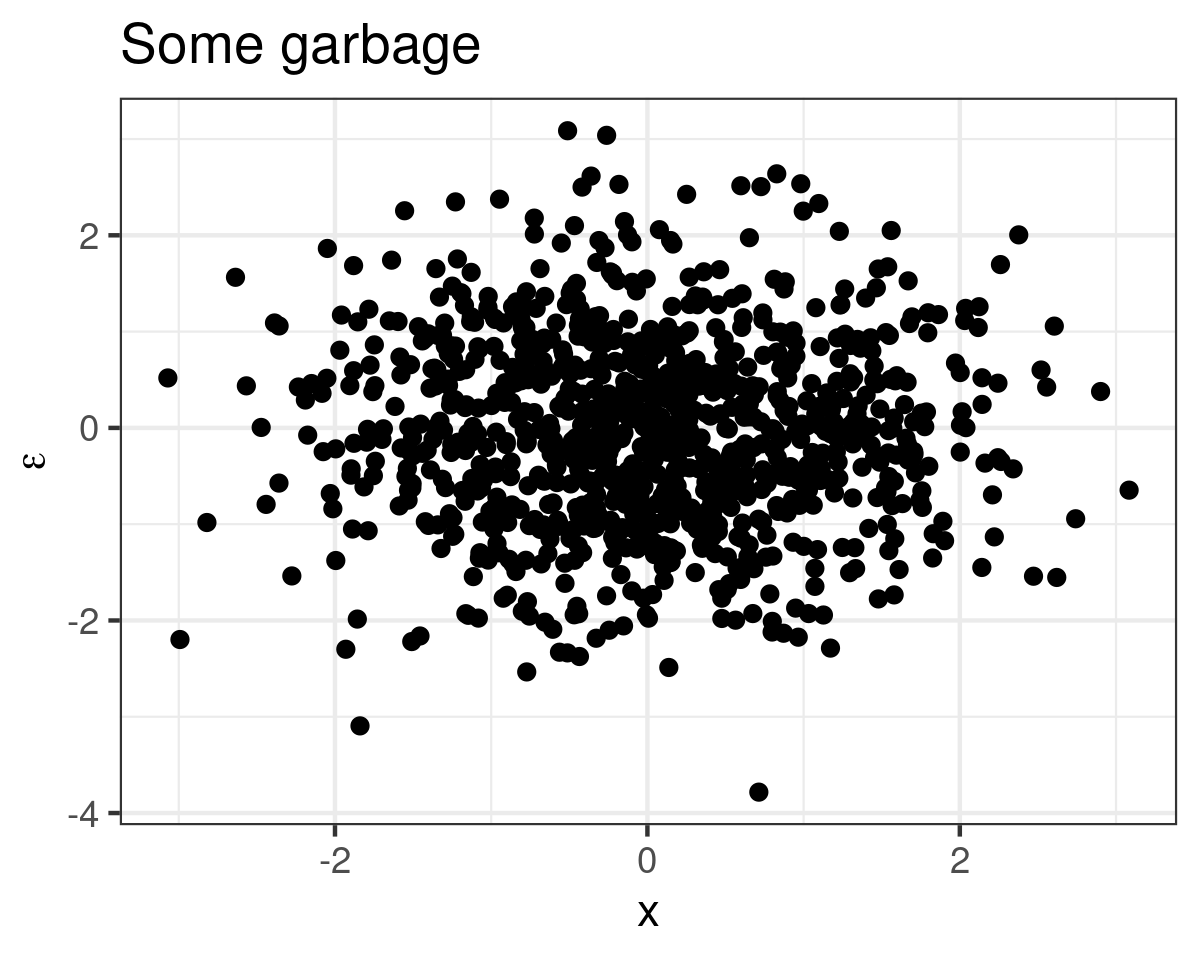
\includegraphics[width=0.980\linewidth,height=0.784\linewidth]{figure/eone_scatter-1} 

}

\caption[It's nice to have a long figure caption that allows easy access to latex stuff like there were $\EoneNumObs$ draws of $x$ and $\epsilon$ that went into this plot]{It's nice to have a long figure caption that allows easy access to latex stuff like there were $\EoneNumObs$ draws of $x$ and $\epsilon$ that went into this plot.}\label{fig:eone_scatter}
\end{figure}


\end{knitrout}

% Knitr automatically labels figures with fig:chunk_name.
And \figref{eone_hist} as well.  What garbage.

% Note that chunk names cannot be repeated.

\begin{knitrout}
\definecolor{shadecolor}{rgb}{0.969, 0.969, 0.969}\color{fgcolor}\begin{figure}[!h]

{\centering 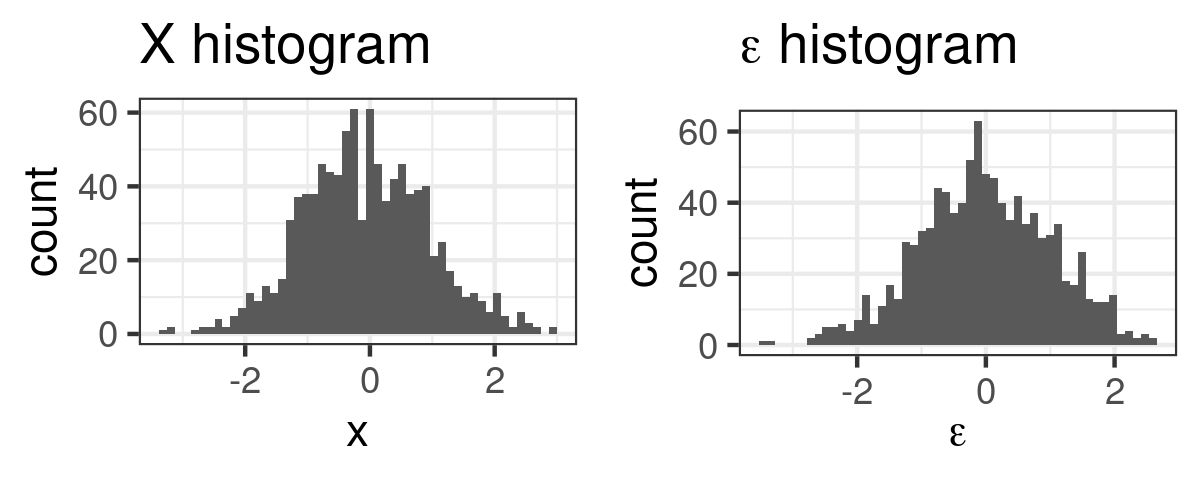
\includegraphics[width=0.980\linewidth,height=0.392\linewidth]{figure/eone_hist-1} 

}

\caption[You can reuse this variable for other captions]{You can reuse this variable for other captions.}\label{fig:eone_hist}
\end{figure}


\end{knitrout}
%
